\documentclass[conference]{IEEEtran}
% \IEEEoverridecommandlockouts
% The preceding line is only needed to identify funding in the first footnote. If that is unneeded, please comment it out.
\usepackage{cite}
\usepackage{amsmath,amssymb,amsfonts}
\usepackage{algorithmic}
\usepackage{graphicx}
\graphicspath{ {./analysis} }
\usepackage{textcomp}
\usepackage{xcolor}
\usepackage{booktabs}
\usepackage{tabularx}
\usepackage{hyperref}
\def\BibTeX{{\rm B\kern-.05em{\sc i\kern-.025em b}\kern-.08em
    T\kern-.1667em\lower.7ex\hbox{E}\kern-.125emX}}
\begin{document}

\title{Comparing Hyperdimensional Computing to Deep Learning for Natural Language Processing Tasks}

\author{\IEEEauthorblockN{Todd Morrill}
\IEEEauthorblockA{\textit{Computer Science Department} \\
\textit{Columbia University}\\
tm3229@columbia.edu}
\and
\IEEEauthorblockN{Satyam Sharma}
\IEEEauthorblockA{\textit{Computer Science Department} \\
\textit{Columbia University}\\
ss6522@columbia.edu}
}

\maketitle

\begin{abstract}
    Deep learning require large quantities of training data and is both memory and energy intensive, making it impractical for many low-resource devices. In this work, we explore the properties of a neuro-inspired approach called hyperdimensional computing (HDC), which addresses some of the shortcomings of deep learning models. In particular, we compare 
    \begin{enumerate}
        \item Training and inference time
        \item Test set accuracy with respect to training set size
        \item FLOP and memory usage
        \item Robustness to text corruption    
    \end{enumerate}
    in the context of a natural language processing (NLP) classifier and show that HDC excels in nearly all of these categories.
\end{abstract}

\begin{IEEEkeywords}
hyperdimensional computing, HDC, deep learning, natural language processing, NLP
\end{IEEEkeywords}

\section{Introduction}
% Introduce the problem you are solving and motivation behind it
Deep learning is currently the dominant approach in natural language processing (NLP). In particular, the Transformer \cite{Transformer} architecture has been shown to be effective for a wide range of NLP tasks, including language modeling (i.e. next word prediction), document retrieval, and document classification \cite{SuperGLUE}. However, deep learning models require a large amount of training data and are often memory and energy intensive, which limit their usability on low-resource devices (e.g. smartphones). Hyperdimensional computing (HDC), on the other hand, is a neuro-inspired approach to machine learning that is memory and energy efficient and may require far less training data to achieve suitable levels of accuracy \cite{HDC}. In short, HDC typically represents data as random high dimensional vectors (e.g. a word may be represented in $\{-1, 1\}^{10,000}$). Each vector might be analagous to a ``thought-vector'' corresponding to some activation of neurons in the brain. HDC uses a variety of elementwise operations to operate on this data. In particular, the bundling operation is elementwise vector addition, the binding operation is elementwise multiplication, the permutation is a rotation of coordinates (i.e. shift to the left), and comparison can be done using a hamming distance or cosine similarity. These operations allow HDC to perform next word prediction, document retrieval, and classification, among other tasks.\\
\\
In this project, we experiment with a commonly used deep learning model for resource constrained settings, the \verb|distilbert-base-uncased| transformer model \cite{sanh2020distilbert}. We compare this deep learning model to an HDC model for an NLP classification task, namely language identification, where the task is to identify which of 21 European languages \cite{quasthoff-etal-2006-corpus} a text example belongs to. We evaluate both models using a range of metrics and evaluate their relative strengths and weaknesses.

% show some sample data with line wrapping
\begin{table}[htbp]
\caption{Sample data from the language identification dataset, which contains 21 European languages.}
\begin{center}
    \begin{tabularx}{\columnwidth}{XX}
\toprule
Language & Example \\
\midrule
English & for denmark and the united kingdom the relevant protocols to the treaty make explicit reference to the socalled opting in and opting out \\
Bulgarian & iskam sshcho taka da podchertaia che nastoiashchata preporka kategorichno shche zasili motivatsiiata za razvitie na predpriemachestvoto sred zhenite \\
Slovak & musite zostrojit graf so znazornenim sposobu akym mozno zapricinuje oteplovanie \\
Portuguese & em meu entender esta reforma nao foi por acaso que o colega pomes ruiz falou do regulamento financeiro e por assim dizer uma quimera ha dois anos que dela se fala mas pareceme que todas as propostas estao a levantar dificuldades e toda uma serie de problemas \\
Czech & evropske pravni pozadavky na spravedlive primerene a zakonne zpracovani osobnich udaju maji rozhodujici vyznam a musi byt vzdy dodrzovany \\
French & la commission a alloue des centaines de millions daide durgence aux populations les plus affectees \\
\bottomrule
\end{tabularx}

\end{center}
\label{tab:examples}
\end{table}

\section{Models and Data Set Description}
\label{sec:models}
We used Python for our implementation and used PyTorch and Hugging Face \cite{HF} to implement the deep learning models and TorchHD \cite{torchhd} to implement the HDC models. \verb|distilbert-base-uncased| is a commonly used lightweight transformer model, that is 40\% smaller than BERT (110 million parameters to  66 million), 60\% faster than BERT, and retains 97\% of its language understanding capabilities \cite{sanh2020distilbert} and as the name implies was trained using knowledge distillation, with BERT as the teacher model. We believe this is a natural deep learning model architecture for comparison to HDC since the authors specifically built this model with resource-constrained settings in mind (e.g. mobile devices).\\
\\
The HDC model was inspired by the architecture found in \cite{HDC}. The model defines a vocabulary of 28 elements, which contains all characters \verb|a| through \verb|z| plus a space and padding character. Each character is initialized with a random 10,000 dimensional vector in $\{\pm 1\}^{10,000}$. High dimensional spaces have been shown to have useful mathematical properties such as near orthogonality of all such randomly generated vectors. The HDC model uses a tri-gram character model which generates sentence embeddings as follows. For each sentence, we generate a sequence of tri-grams, where each tri-gram is the concatenation of three consecutive characters in the sentence. These 3 letters each have a 10,000 dimensional vector that represent it. We then use the permutation operation, which shifts the elements of the first chararacter's embedding to the left 2 positions, shifts the elements of the second character's embedding to the left 1 position, and doesn't shift the third character's embedding at all. Importantly, this permutation operation helps the model distinush tri-grams from one another by breaking the commutativity of addition and multiplication (see next few sentences). Next, we apply the binding operation, which is the elementwise multiplication of the 3 10,000 dimensional vectors. Finally, we bundle (i.e. add) all the tri-grams in a sentence to obtain a sentence embedding. In particular, we implement

\begin{align}
    \bigoplus_{i=0}^{m - n} \bigotimes_{j = 0}^{n - 1} \Pi^{n - j - 1}(V_{i + j}) \label{eq:embedding}
\end{align}

where $\prod$ denotes the permutation (i.e. roll) operator, $\otimes$ denotes the binding operator, and $\oplus$ denotes the bundling operator. In order to keep the precision of the sentence embeddings low (i.e. in the set $\{\pm 1\}$) we quantize the resulting sentence embedding with the function

\begin{align}
    q(x) = \begin{cases}
        +1 & \text{if } x \geq 0\\
        -1 & \text{if } x < 0.
    \end{cases}
\end{align}
Training the model is performed as follows. Each sentence embedding (which has a ground truth language associated to it) will be added to the appropriate langugage ``prototype'' vector. The prototype vectors are initialized as 21 zero vectors for the 21 languages. The model is trained by adding sentence embeddings to these prototype vectors. At the end of training, the 21 language vectors are normalized so that they are all unit vectors, which removes any bias due to some classes having more examples than others. The model is evaluated by computing the cosine similarity between the test set sentence embeddings and each of the 21 prototype vectors and selecting the language with the highest similarity score.\\
\\
We train both models on the Wortschatz European language corpus \cite{quasthoff-etal-2006-corpus}. The training dataset contains 210,032 training examples and 21,000 test examples across 21 Europan languages (Bulgarian, Czech, Danish, Dutch, German, English, Estonian,
 Finnish , French , Greek, Hungarian, Italian, Latvian,
Lithuanian, Polish, Portuguese, Romanian, Slovak, Slovenian,
Spanish, Swedish).

\section{Training and Profiling Methodology and Experimental Results}
Our primary objective for this project was to benchmark a commonly used deep learning model against an HDC model on 4 key dimensions:
\begin{enumerate}
    \item Training and inference time
    \item Test set accuracy with respect to training set size
    \item FLOP and memory usage
    \item Robustness to text corruption.
\end{enumerate}

Figures \ref{fig:speed_train} and \ref{fig:speed_test} show an incredible difference in time taken for one epoch of the training and test set, respectively, when running on an NVIDIA Tesla T4 GPU with a batch size of 32. Training time takes 1,559 seconds for the deep learning model and 101 seconds the HDC model, which is a 15x speedup. We will explain why there is such a discepancy when we adress FLOP and memory usage.\\
\\
We then looked at test set accuracy with respect to training set size. We varied the dataset size from 0.01\% of the training dataset all the way up to its full size. Figure \ref{fig:data_size} shows the results of that experiment and HDC demonstrates strong few-shot behavior. In other words, it largely outperforms the deep learning model when the training set size is small and it isn't until the training set size is 10\% of the full training set that the deep learning model begins to outperform HDC, albeit only marginally. It is interesting to note, however, that backpropagation seems to provide a much stronger learning signal that allows the deep learning model to continue to refine itself, whereas the HDC model saturates rather quickly and doesn't seem to be able to improve any futher. Future work might investigate better learning mechanisms in HDC models.\\

\begin{figure}[htbp]
\centerline{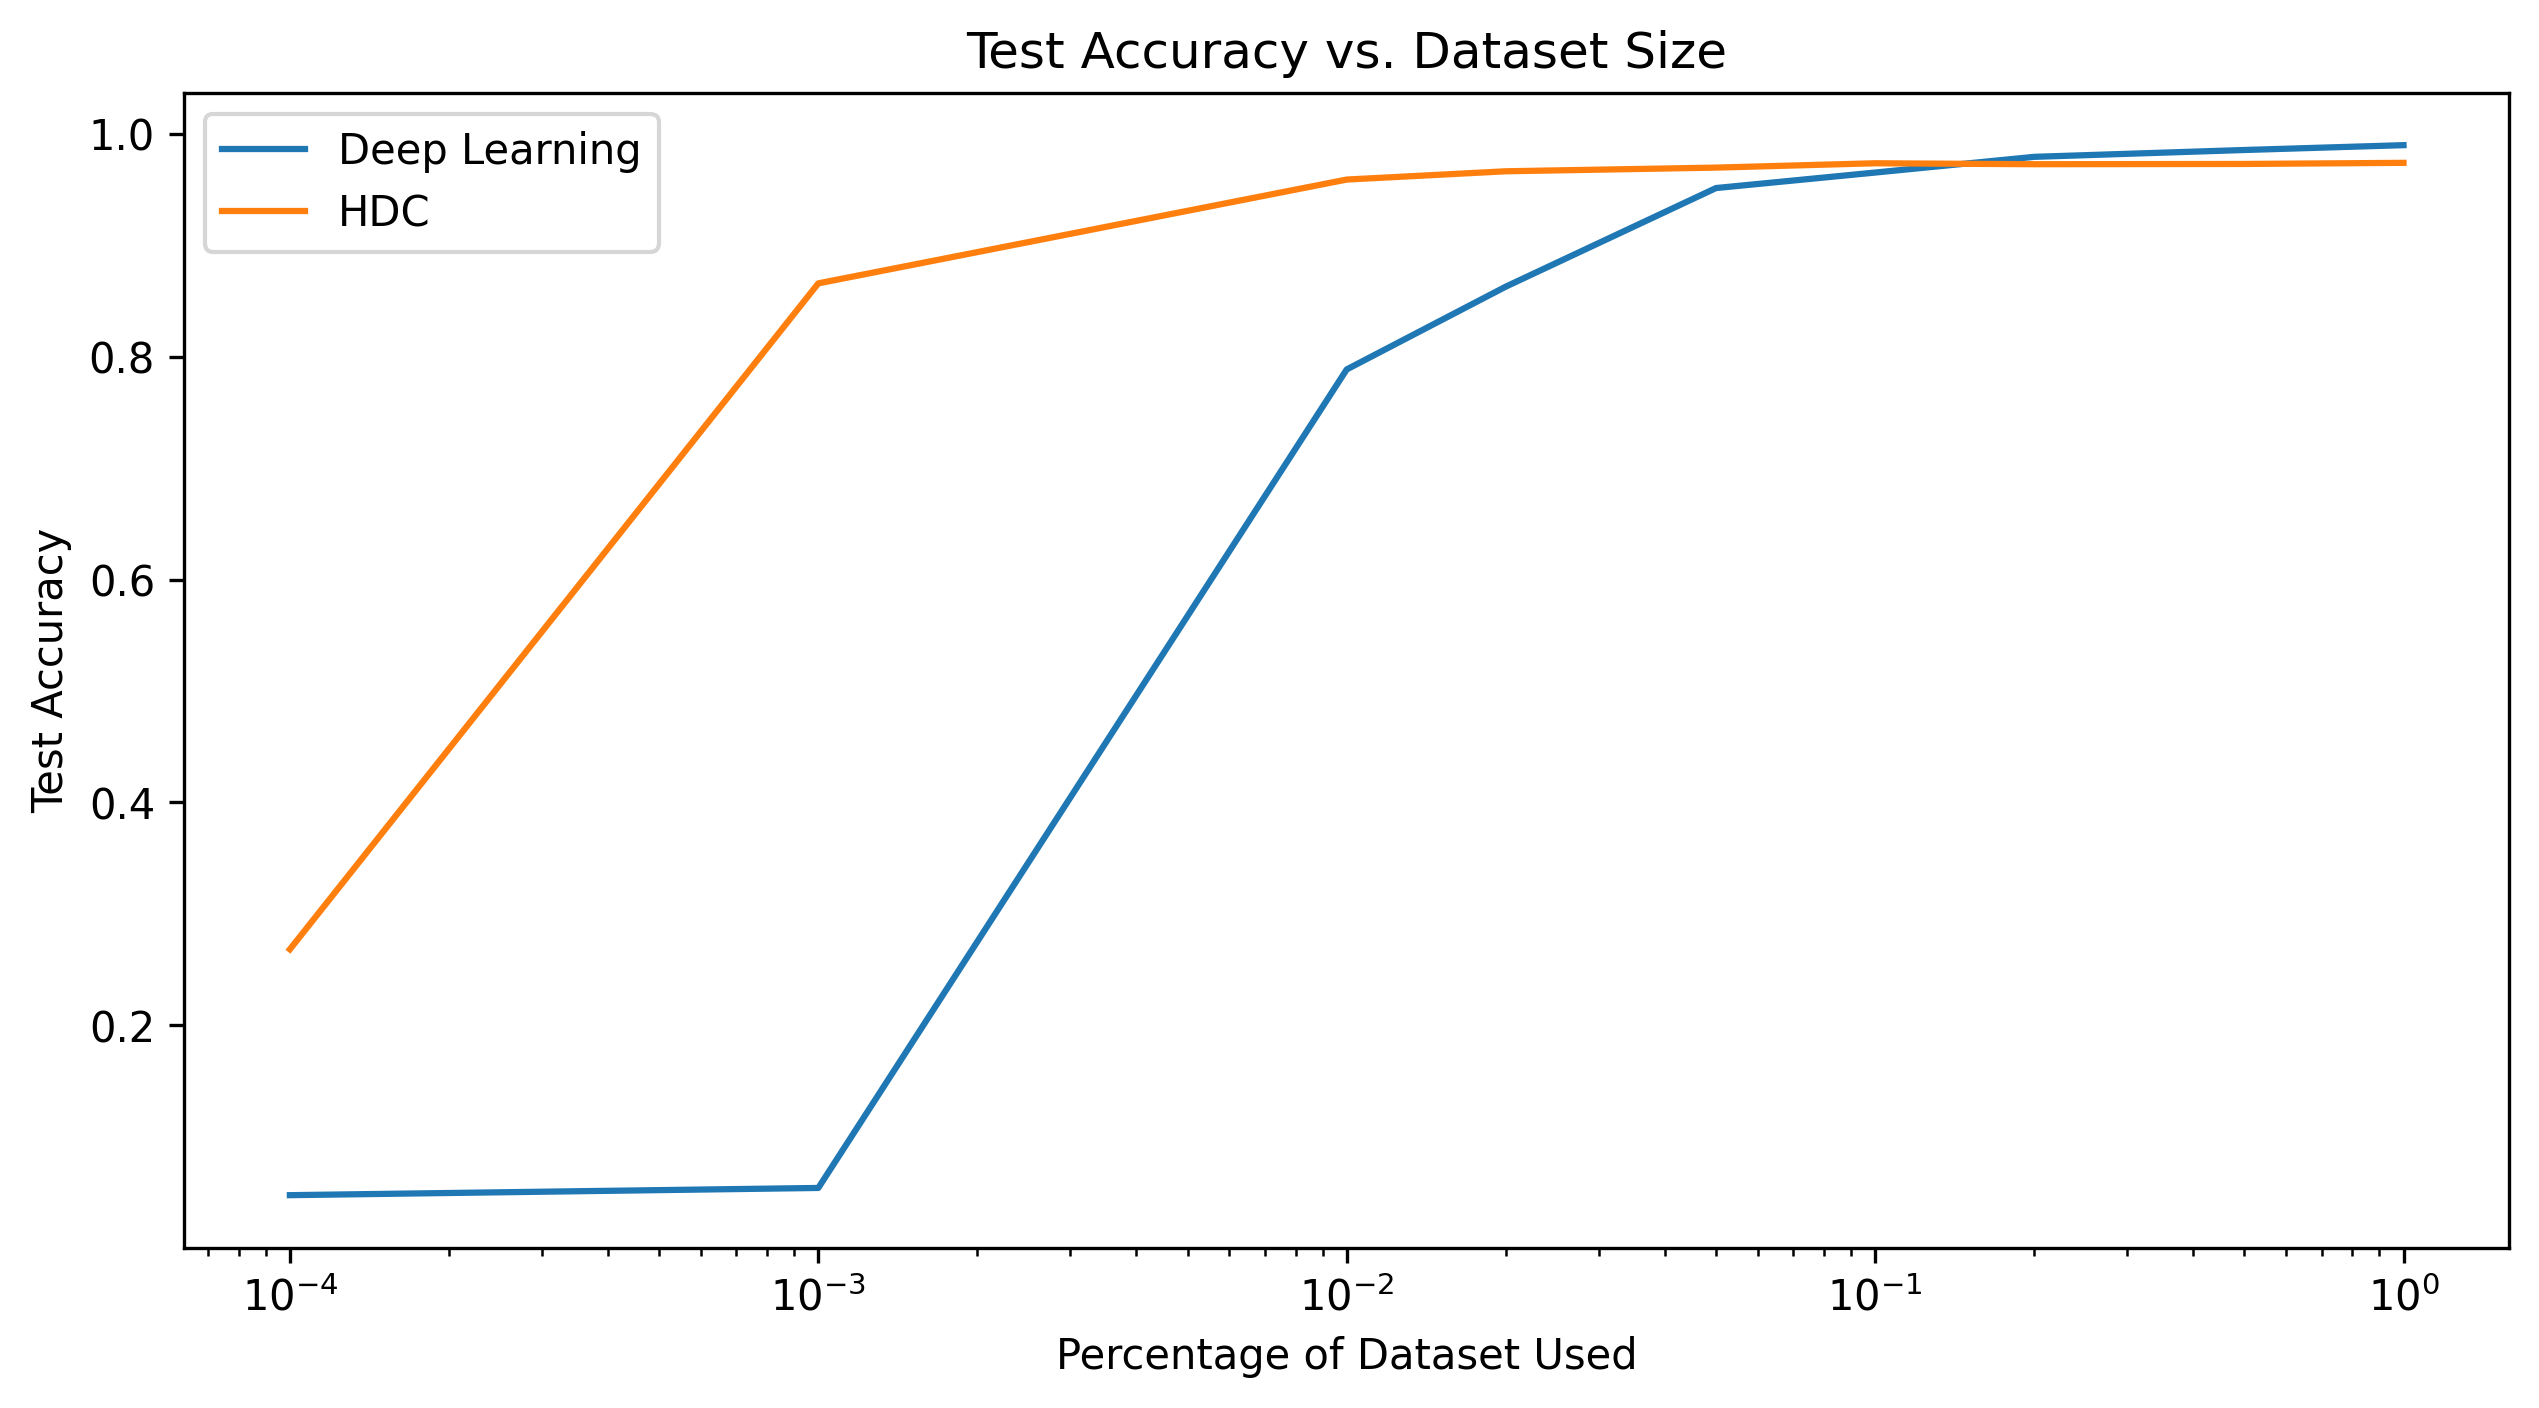
\includegraphics[width=0.5\textwidth]{analysis/data_size.png}}
\caption{Test set accuracy with respect to training set size.}
\label{fig:data_size}
\end{figure}

We then investigated the FLOP and memory usage of the two models. Table \ref{tab:models} shows the number of FLOPs required by a forward pass of the model on a single example and the parameter count includes the number of model parameters in memory. We Facebook AI's \verb|fvcore| library\footnote{\url{https://github.com/facebookresearch/fvcore}} for deriving these results. The discrepancy in both FLOP and memory usage is what accounts for the difference in running times. In particular, the running time of a transformer model is $O(n^2)$ in the length of the input sequence $n$ due to the self-attention mechanism, while the running time of the HDC model is only $O(n)$ because it only needs to encode the sentence and compare it to a fixed set of class prototype vectors. This leads to very interpretable results. In particular, the 210,000 HDC FLOPs correspond to the cosine similarity calculations against the 21 prototype vectors, each of which is a 10,000 dimensional vector. The number of parameters (490,000 = 210,000 + 280,000) corresponds to the 21 prototype vectors, each of which is a 10,000 dimensional vector, plus the 28 character vectors, each of which is a 10,000 dimensional vector. Again, we note that the HDC model delivers performance matching the deep learning model with a fraction of the deep learning model's 43,135,509 parameters.\\

\begin{table}[htbp]
\caption{FLOP and memory usage of the two models.}
\centering
\label{tab:models}
\begin{tabular}{ccc}
\toprule
Model & Parameters & FLOPs \\
\midrule
HDC & 490000 & 210000 \\
distilbert-base-uncased & 43135509 & 936371712 \\
\bottomrule
\end{tabular}

\end{table}

Our final experiment was to test the robustness of the two models to text corruption. Many HDC papers note its robustness to corruption of its internal memory mechanisms, but fewer works address the models' robustness to corruption of the input. We defined the following corruption scheme for the test set. We define a corruption rate, and for each character in the sentence, we randomly decide whether to corrupt it or not. If we decide to corrupt it, we choose uniformly over the following action set to corrupt that character:
\begin{enumerate}
    \item Insert a random character
    \item Delete the character
    \item Substitute the character with a random character
    \item Swap the character with the next character.
\end{enumerate}

We tested the models on the test set while varying the corruption rate. The results are shown in Figure \ref{fig:robustness}. We again show that the HDC model outperforms the deep learning model in this regard. As the corruption rate is increased, we see the performance of the deep learning model decline faster than the HDC model, indicating a higher degree of robustness to corrupted text input of the HDC model.

\begin{figure}[htbp]
\centerline{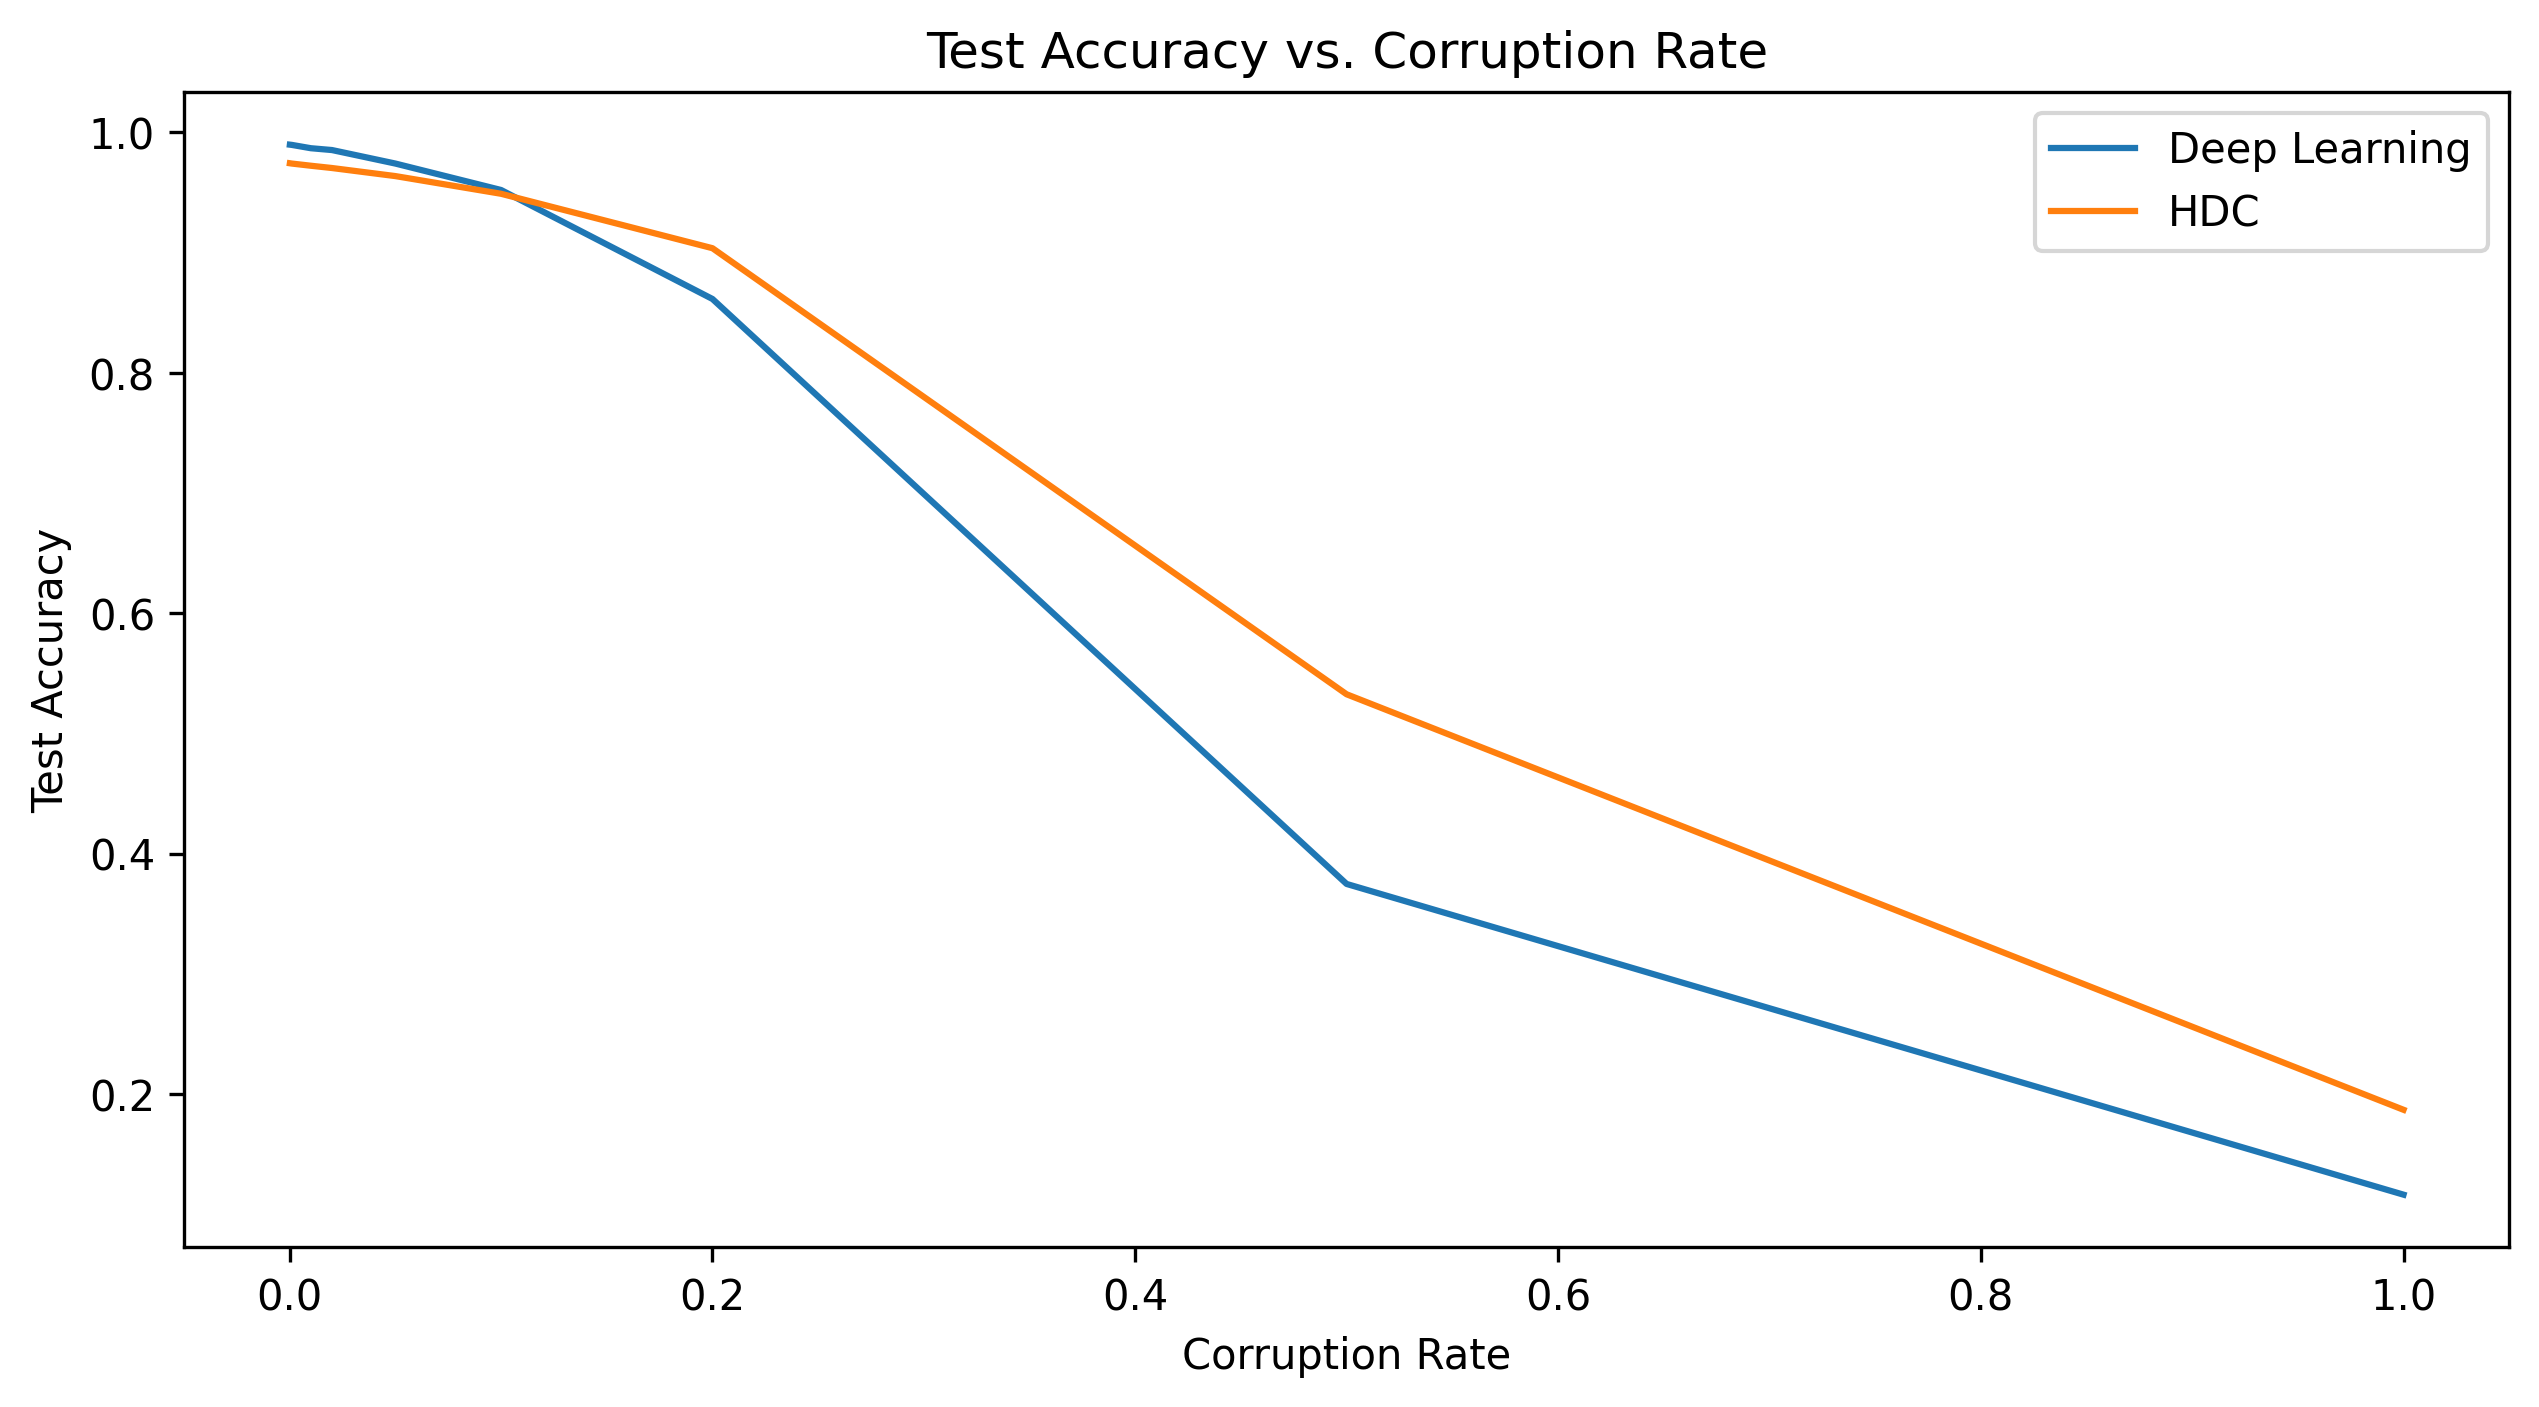
\includegraphics[width=0.5\textwidth]{analysis/corruption.png}}
\caption{Test set accuracy with respect to corruption rate.}
\label{fig:robustness}
\end{figure}

\section{Performance Tuning Methodology}
While tuning was not the primary objective of this project, we did find one opportunity for performance improvement. In particular, we after profiling the HDC model using the \verb|torch.profiler| we found that the HDC model was spending a significant amount of time in the \verb|torch.roll| function, which is responsible for the shifting of vector elements to the left by 1 or 2 elements as described in Section \ref{sec:models}. This function must shift all elements of a vector, which we know will require an enormous number of memory accesses to carry out. Taking inspiration from the way that convolutions were described in class, we implemented a ``roll matrix'', which looks like the following:
\begin{align}
    \begin{bmatrix}
    0 & 0 & 1 \\
    1 & 0 & 0 \\
    0 & 1 & 0
    \end{bmatrix},
\end{align}

which is corresponds to rolling by 1 dimension. Instead of focusing on rolling the entire 10,000 dimensional vector, we only rolled the last 3 dimensions.

\begin{figure}[htbp]
    \centering
    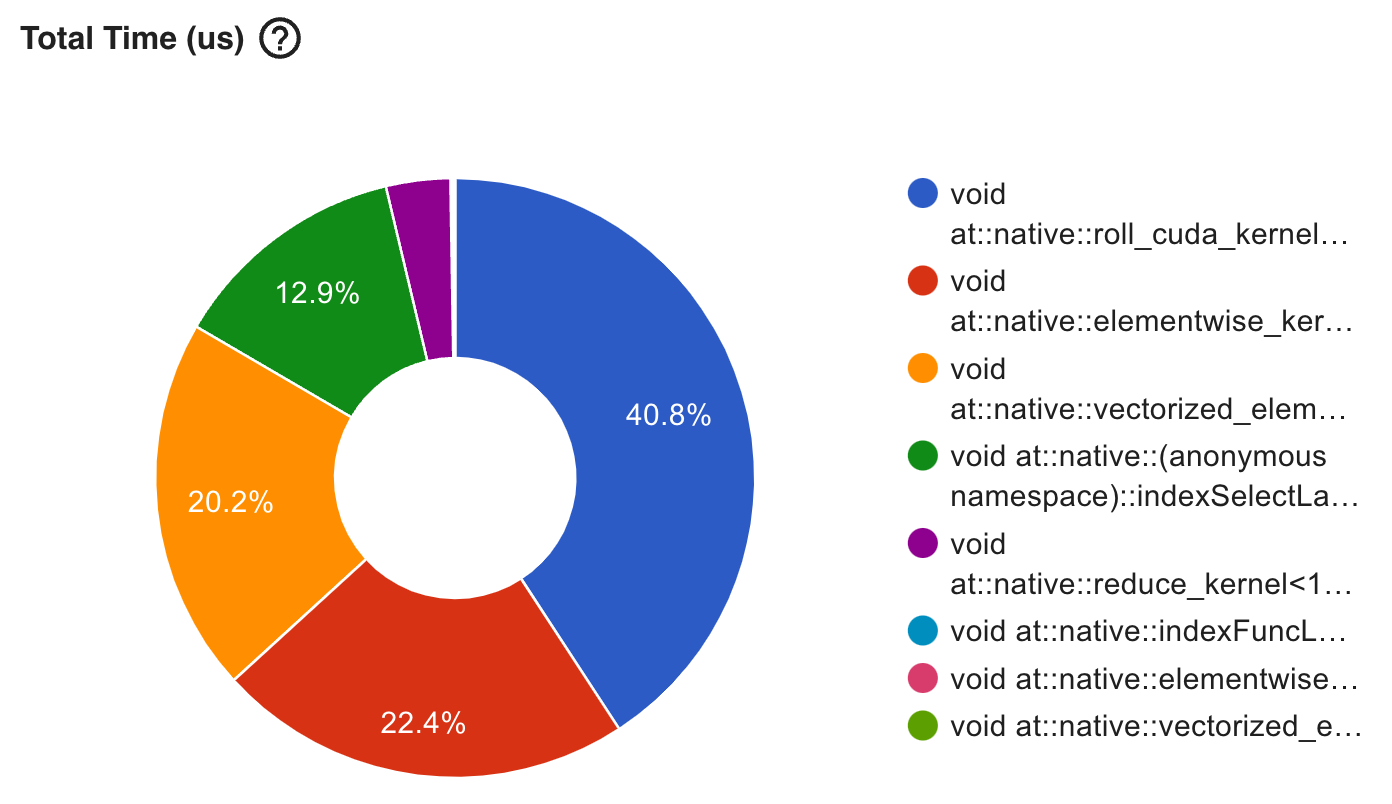
\includegraphics[width=0.5\textwidth]{./analysis/torch_roll.png}
    \caption{We note the blue portion of the pie chart denoting the torch.roll operation, which dominates the HDC runtime.}
    \label{fig:roll}
\end{figure}

\begin{figure}[htbp]
    \centering
    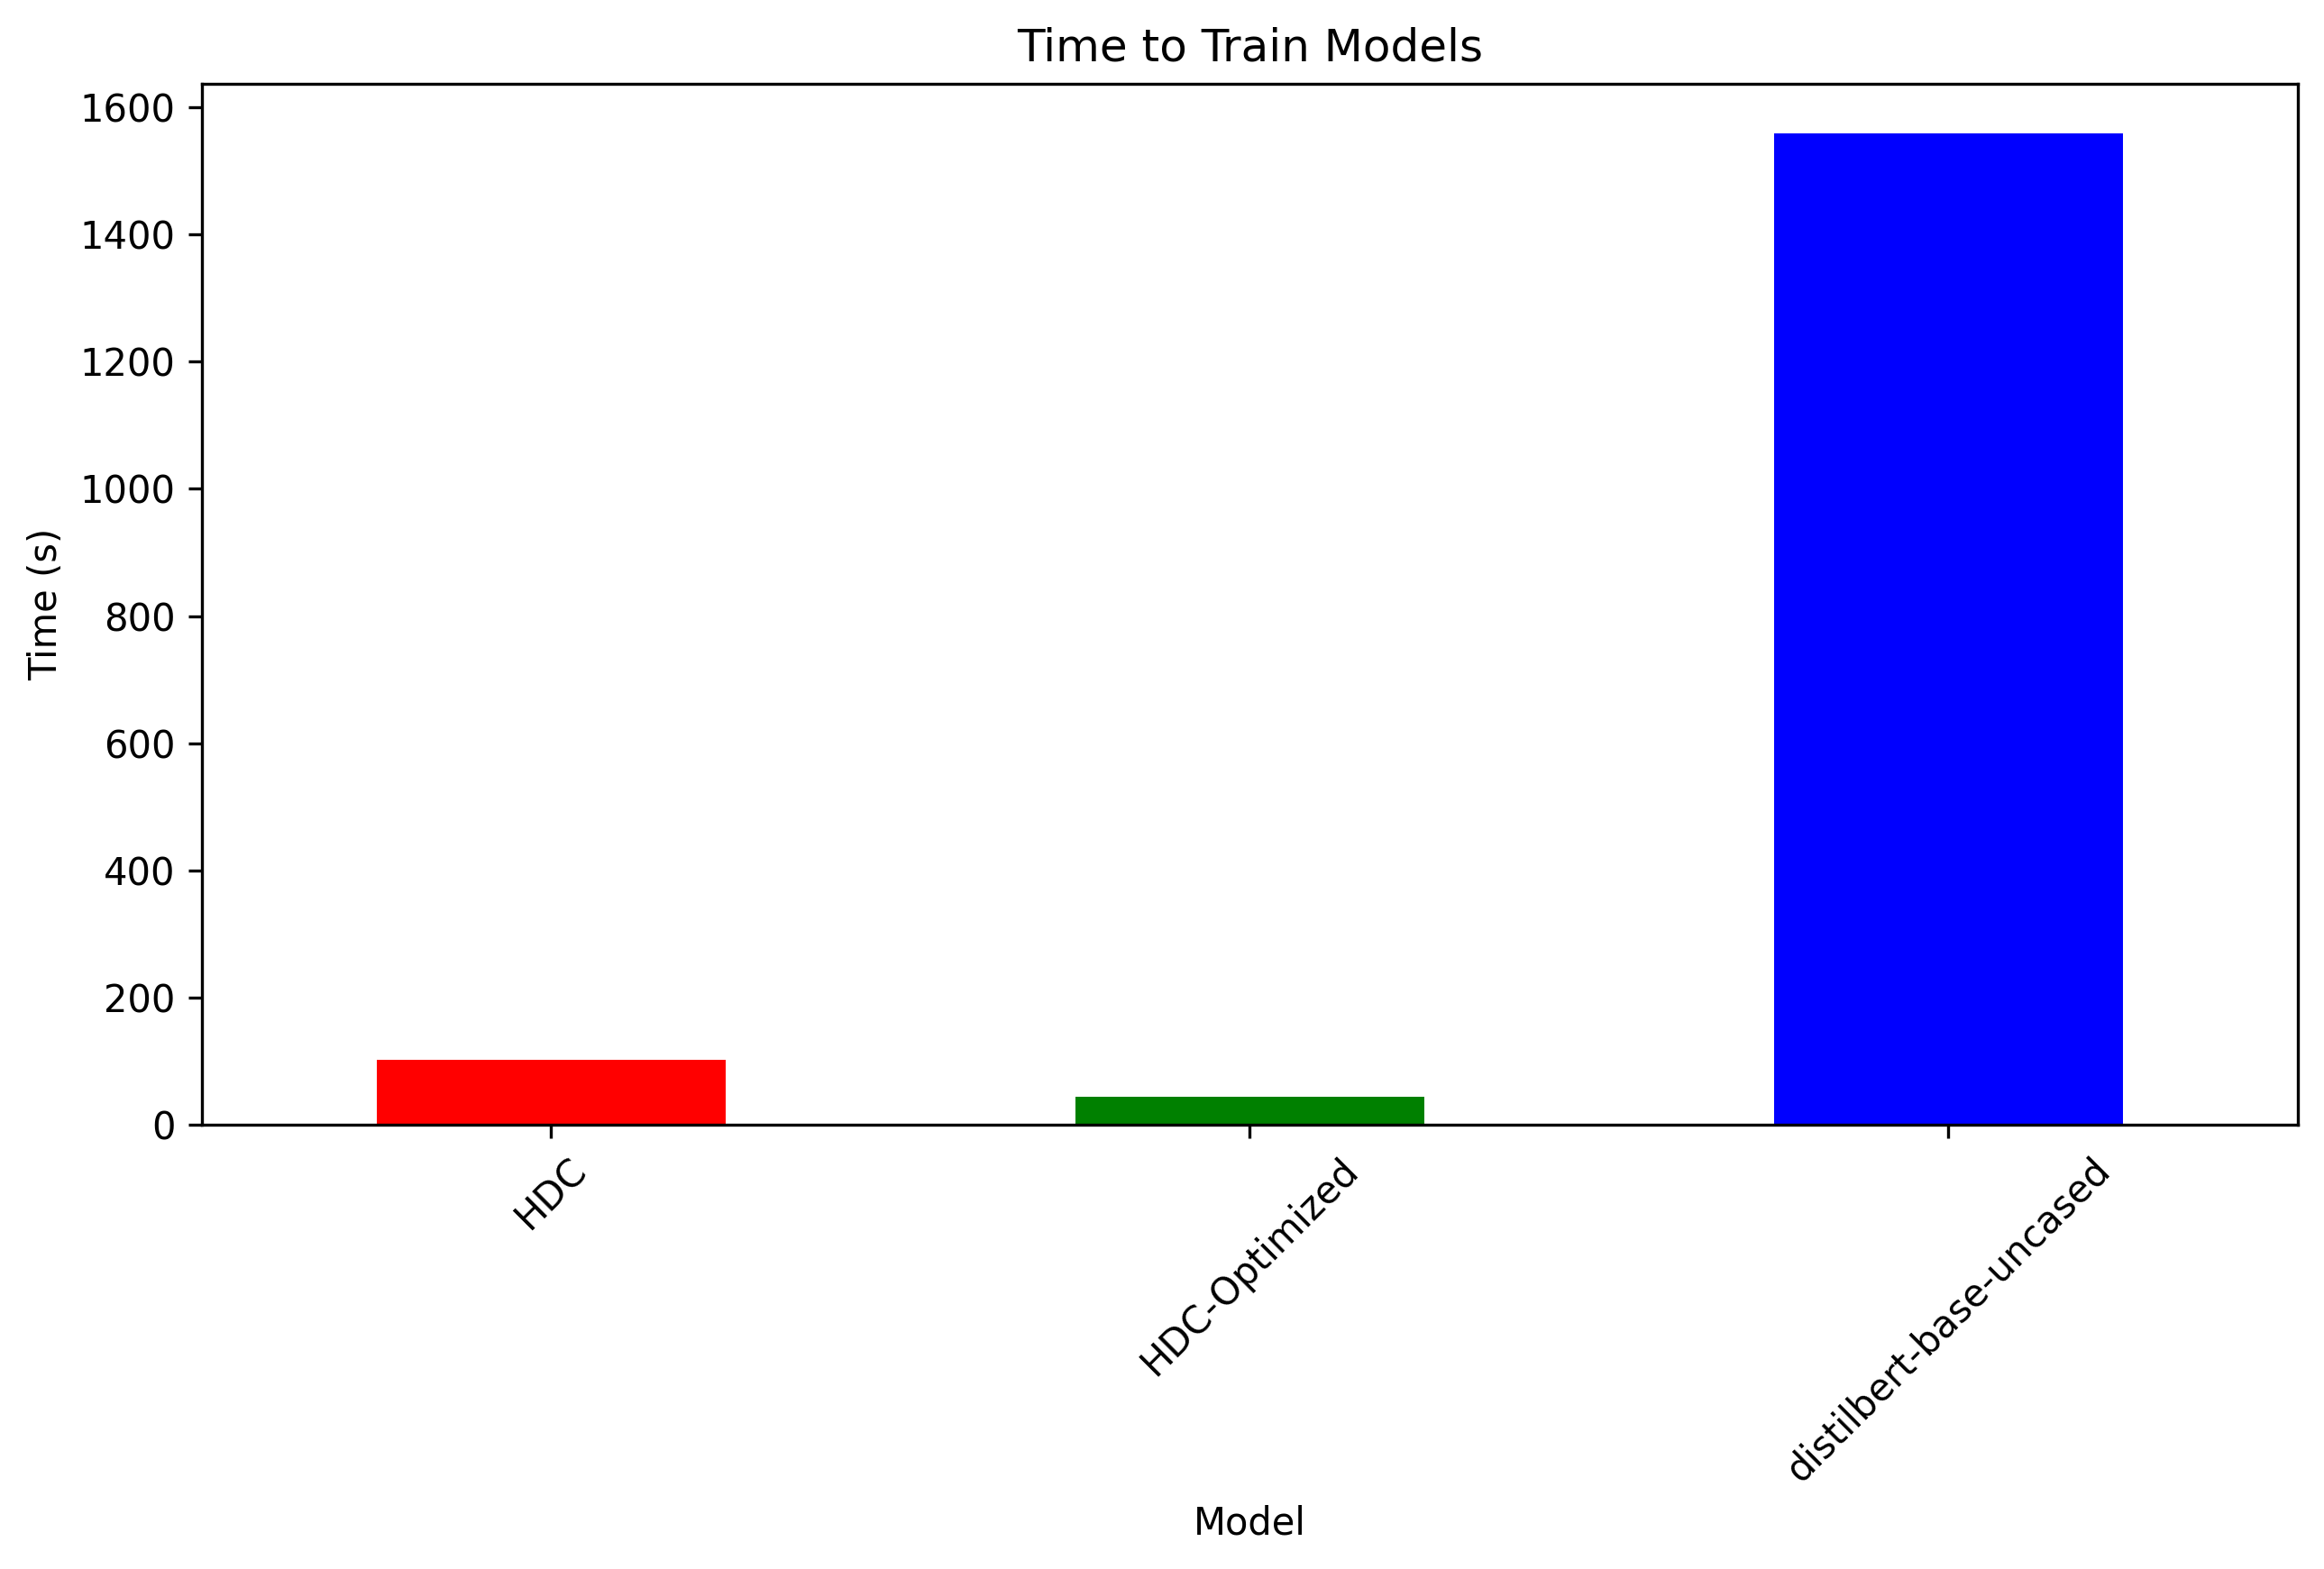
\includegraphics[width=0.5\textwidth]{./analysis/speed_train.png}
    \caption{Training times for one epoch using the baseline HDC model, optimized HDC model, and the deep learning model.}
    \label{fig:speed_train}
\end{figure}

\begin{figure}[htbp]
    \centering
    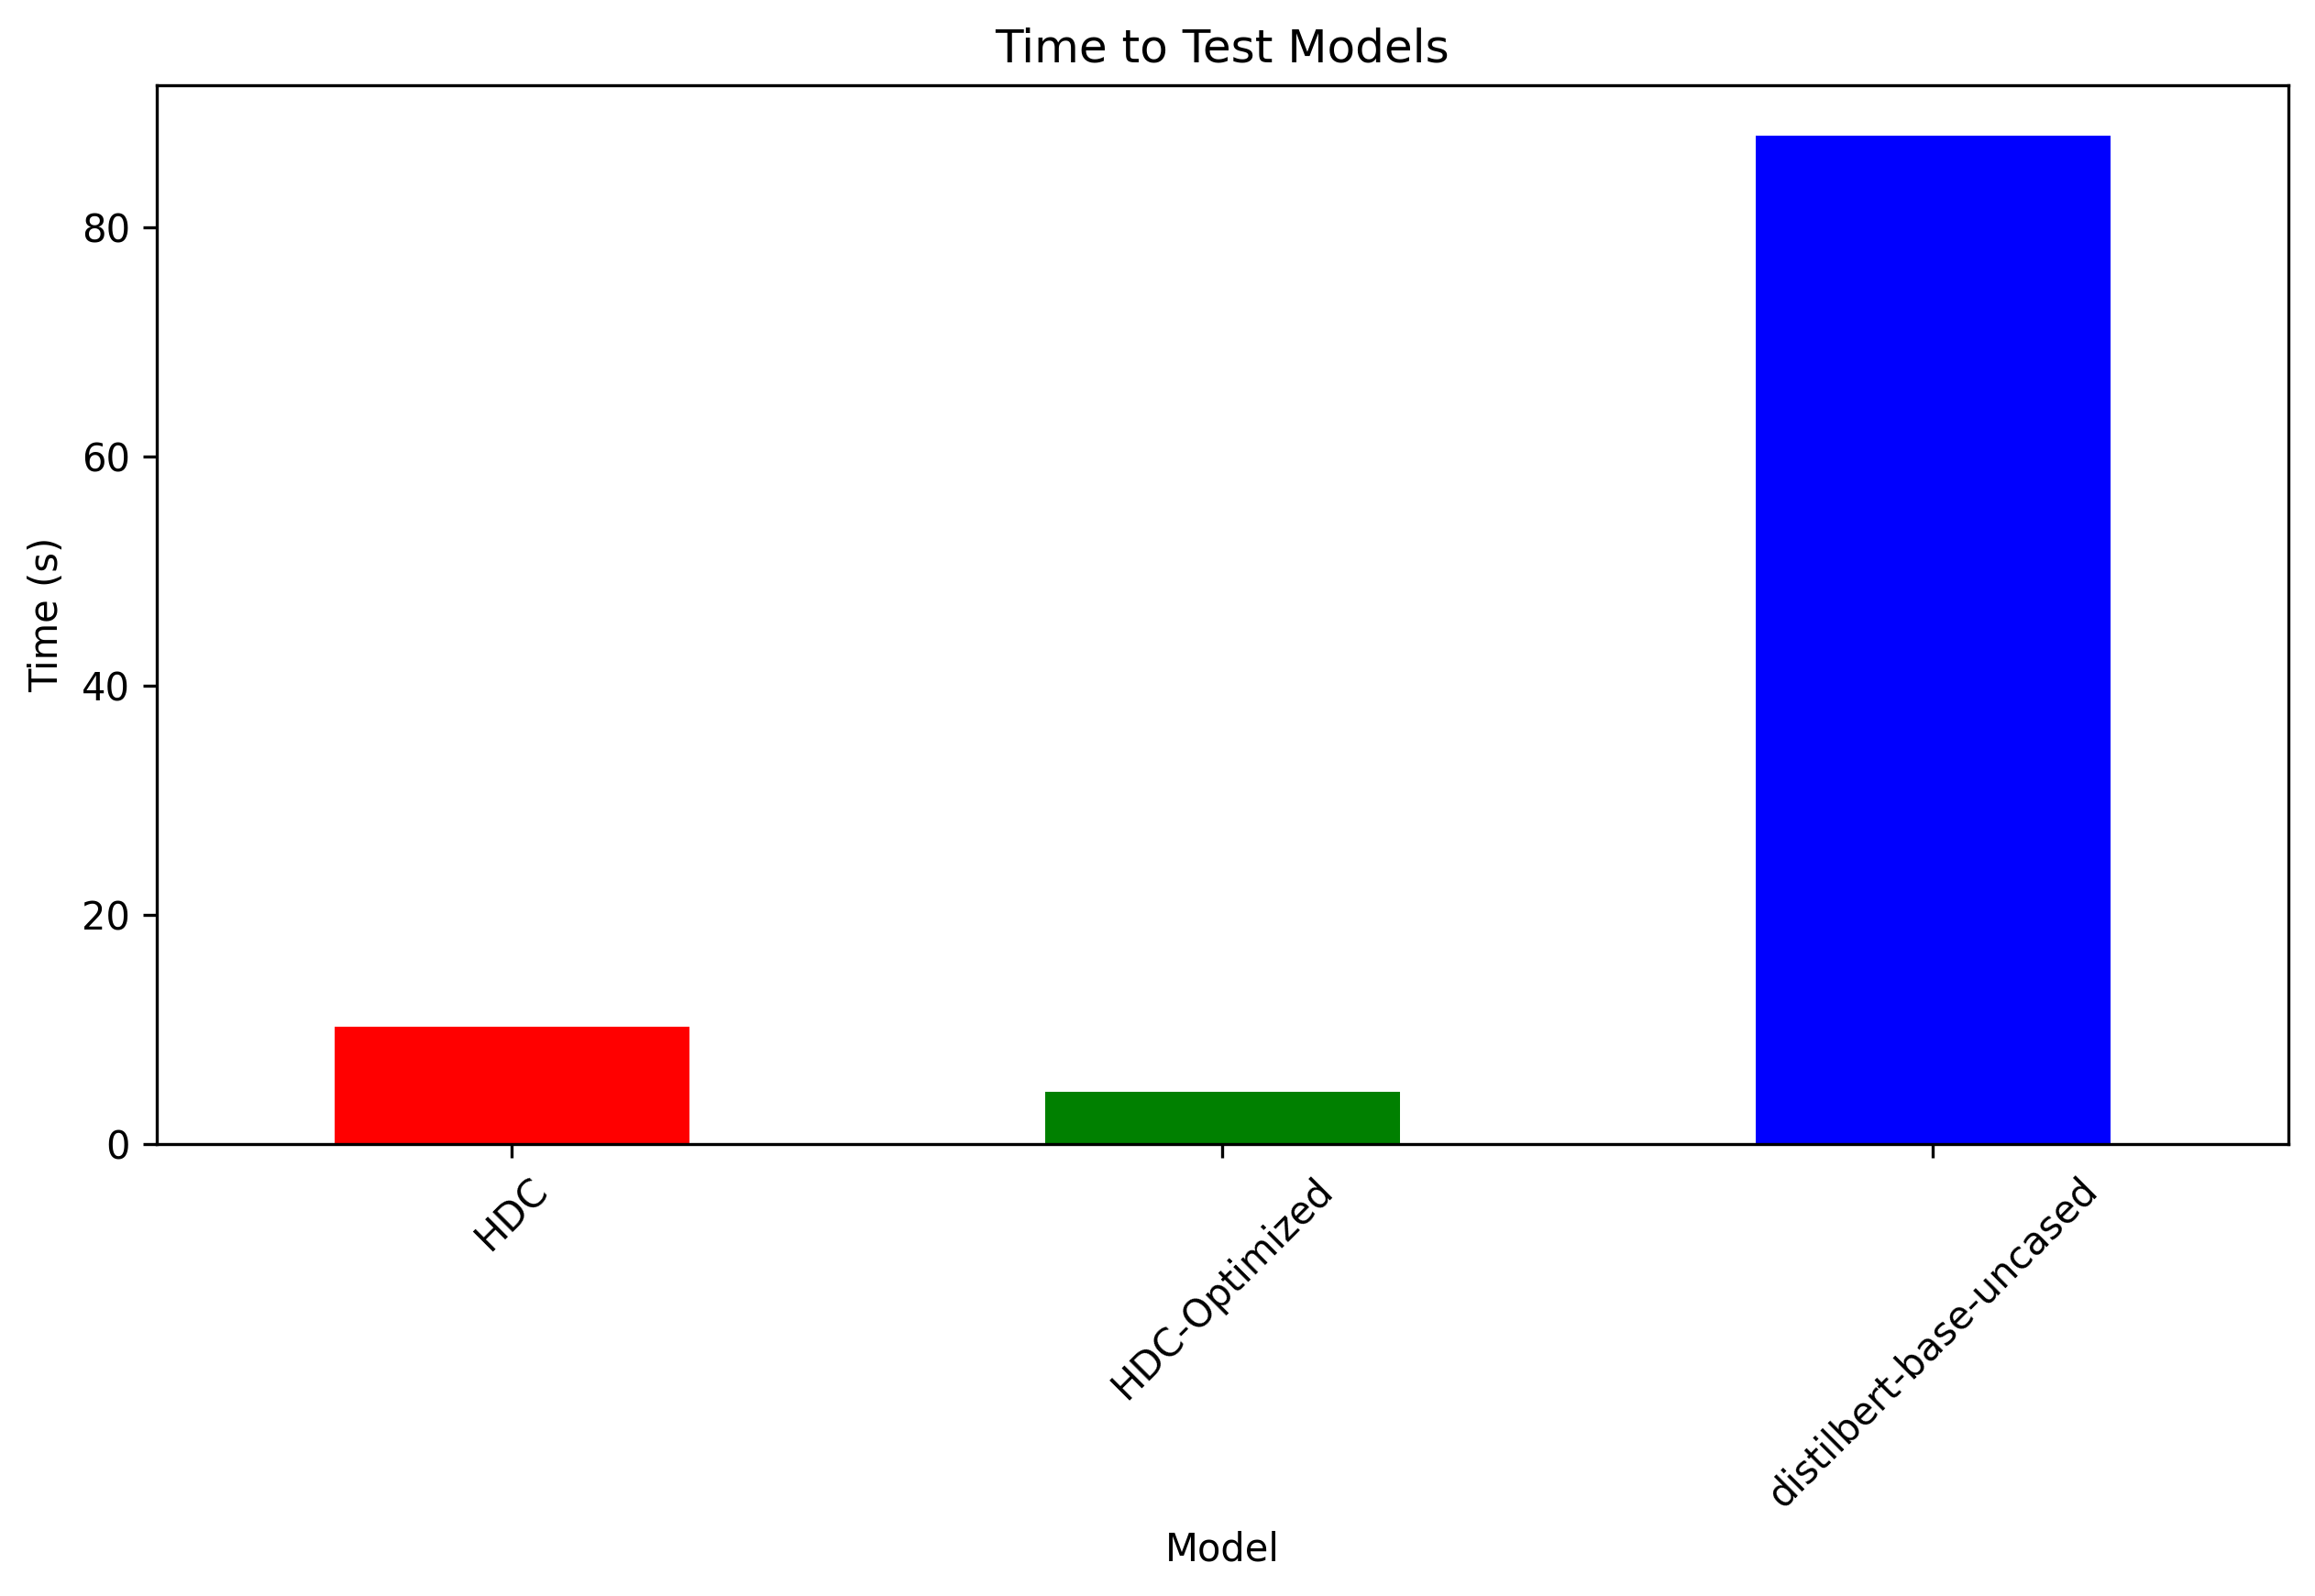
\includegraphics[width=0.5\textwidth]{./analysis/speed_test.png}
    \caption{Inference times on the test set for one epoch using the baseline HDC model, optimized HDC model, and the deep learning model.}
    \label{fig:speed_test}
\end{figure}

Figure \ref{fig:roll} shows the \verb|torch.profiler| results that tipped us off to the bottleneck. Figures \ref{fig:speed_train} and \ref{fig:speed_test} show the running time comparison for one epoch of data before and after implementing this optimization. After implementing the described roll matrix, we obtain more than a 2x speedup, albeit at a slight cost of accuracy, which declines to about 90\% from about 98\%. At a minimum, it is useful to be aware of this choice that a developer has to sacrifice a small amount of accuracy in exchange for a faster runtime.

\section{Conclusion}
We have shown that the HDC model is a viable alternative to deep learning models for text classification tasks. We have shown that the HDC model is more robust to corruption of the input text, and that it is more efficient in terms of memory usage and runtime. We have also shown that the HDC model is more accurate than the deep learning model when the dataset size is small. Future work can determine how applicable HDC models are to other natural language tasks. For example, there are very natural extensions to this work for approximate nearest neighbor seach for document retrieval. It's also possible that the HDC model can be extended to other tasks such as machine translation or question answering though suitable next word prediction schemes must be devised. Our model was incredibly efficient because we only materialize a codebook for 28 characters, however, if we had to retain a larger codebook (e.g. for a vocabulary of size 30,000 or more), we would start running into issues with memory. Future work can investigate how to efficiently handle larger codebooks. Finally, we note that the HDC models are shallow, essentially single layer encoder-decoder models. Future work can investigate the performance of deeper HDC models. HDC models also have a rather trivial learning scheme. It would be interesting to investigate other learning schemes for HDC models. In closing, high-dimensional, low precision spaces inspired by the human brain have useful properties that we can exploit to build efficient and accurate models.

\section{Appendix}
% include table
\begin{table}[htbp]
\caption{HDC accuracy scores by dataset size.}
\begin{center}
    \begin{tabular}{ccc}
\toprule
 Examples &  Dataset Pct. &  Accuracy \\
\midrule
       21 &        0.0001 &    0.2682 \\
      210 &        0.0010 &    0.8375 \\
     2100 &        0.0100 &    0.9593 \\
     4200 &        0.0200 &    0.9659 \\
    10501 &        0.0500 &    0.9700 \\
\bottomrule
\end{tabular}

\end{center}
\label{tab:hdc_acc}
\end{table}

\begin{table}[htbp]
    \caption{Deep learning accuracy scores by dataset size.}
    \begin{center}
        \begin{tabular}{ccc}
\toprule
Examples & Dataset Pct. & Accuracy \\
\midrule
21 & 0.0001 & 0.0476 \\
210 & 0.0010 & 0.0541 \\
2100 & 0.0100 & 0.7886 \\
4200 & 0.0200 & 0.8629 \\
10501 & 0.0500 & 0.9513 \\
21003 & 0.1000 & 0.9652 \\
42006 & 0.2000 & 0.9793 \\
105016 & 0.5000 & 0.9855 \\
210032 & 1.0000 & 0.9898 \\
\bottomrule
\end{tabular}

    \end{center}
    \label{tab:dl_acc}
\end{table}

\begin{table}[htbp]
    \caption{Deep learning speed analysis.}
    \begin{center}
        \begin{tabular}{ccc}
\toprule
Model & Training-Time & Testing-Time \\
\midrule
distilbert-base-uncased & 1426507.625000 & 77738.898438 \\
\bottomrule
\end{tabular}

    \end{center}
    \label{tab:dl_speed}
\end{table}

\begin{table}[htbp]
    \caption{Deep learning FLOP analysis.}
    \begin{center}
        \begin{tabular}{ccc}
\toprule
Model & Parameters & FLOPs \\
\midrule
HDC & 490000 & 210000 \\
distilbert-base-uncased & 43135509 & 936371712 \\
\bottomrule
\end{tabular}

    \end{center}
    \label{tab:dl_flop}
\end{table}

\bibliographystyle{IEEEtran}
\bibliography{IEEEabrv, bib.bib}
\end{document}
